\usetikzlibrary{arrows.meta,calc,fit,matrix,shapes,shapes.misc}
\providecommand{\computer}{%
    
\includegraphics[width=1cm]{../common/Noun_project_216.pdf}
}
\providecommand{\computerAlt}{%
    
\includegraphics[width=1cm]{../common/Noun_project_alt_cpu.pdf}
}
\providecommand{\switch}{%
    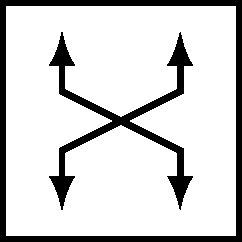
\includegraphics[width=0.9cm]{../common/fig-switch.pdf}
}
\providecommand{\router}{%
    
\includegraphics[width=0.9cm]{../common/fig-router.pdf}
}


\begin{frame}{DNS cache poisoning}
\begin{tikzpicture}
\tikzset{
    computer/.style={inner sep=0mm,outer sep=0mm,execute at begin node={\computer}},
    computer alt/.style={inner sep=0mm,outer sep=0mm,execute at begin node={\computerAlt}},
    connect/.style={draw,very thick,Latex-Latex},
    connect big/.style={draw,ultra thick,Latex-Latex},
    network/.style={cloud,draw,aspect=2},
    marked/.style={draw,line width=1mm,blue,dotted},
    marked pack/.style={draw,solid,line width=0.8mm,draw=blue,fill=white,align=left,
        font=\small},
    marked alt/.style={draw,line width=1mm,violet,dotted},
    marked pack alt/.style={draw,solid,line width=0.8mm,draw=violet,fill=white,align=left,
        font=\small},
};

\node[computer] (attacker) at (0, 2) {};
\node[computer] (attacker2) at (2, -3) {};
\node[font=\huge] at (attacker) {\emoji{smiling-face-with-horns}};
\node[font=\huge] at (attacker2) {\emoji{smiling-face-with-horns}};
\node[computer] (victim) at (0, -2) {};
\node[network] (net) at (3.5, 0) {~~};
\node[network] (net2) at (5, -3) {~~};
\node[computer,label={south:dns.isp.com}] (resolver) at (7, 2) {};
\node[computer,label={south:ns.foo.com}] (authority) at (10, -3) {};
%
\draw[connect] (attacker) -- (net);
\draw[connect] (victim) -- (net);
\draw[connect] (net) -- (net2);
\draw[connect] (net) -- (resolver);
\draw[connect] (net2) -- (authority);
\draw[connect] (net2) -- (attacker2);
%
\begin{visibleenv}<2>
\draw[marked,-Latex] (attacker) -- ([yshift=.1cm]net.center) 
    node[pos=0.25,above right,marked pack] {
        \emoji{smiling-face-with-horns} user $\rightarrow$ dns.isp.com: \\
        foo.com IN A ?
    } -- (resolver.west);
\end{visibleenv}
\begin{visibleenv}<3>
\draw[marked,-Latex] (resolver.south) -- ([yshift=-.1cm]net.center) 
    node[pos=0.35,below right,marked pack] {
        dns.isp.com $\rightarrow$ ns.foo.com: \\
        foo.com IN A ?
    } -- (net2.center) -- (authority);
\end{visibleenv}
\begin{visibleenv}<3>
\draw[marked alt,-Latex] (attacker2) -- ([xshift=-.3cm]net2.center)
    node[pos=0.25,marked pack alt,below right=0.5cm] {
        (`spoofed' by attacker) \\
        ns.foo.com $\rightarrow$ dns.isp.com: \\
        foo.com 9999999 IN A (attcker's IP) 
    }
    -- ([xshift=-.4cm,yshift=.2cm]net.center) -- ([yshift=-.2cm]resolver.west);
\node[anchor=north west,draw=red,ultra thick,align=left,font=\small] at ([xshift=2cm]resolver.north east) {
    attacker's `spoofed' response \\
    causes dns.isp.com to record \\
    wrong IP
};
\end{visibleenv}
\begin{visibleenv}<4>
\draw[marked,-Latex] (victim) -- (net) node[pos=0.25,above right,marked pack] {
       innocent user $\rightarrow$ dns.isp.com: \\
       foo.com IN A ?
}
    -- (resolver.west);

\draw[marked,-Latex] (resolver.south) -- (net) node[pos=0.25,above right,marked pack] {
       dns.isp.com $\rightarrow$  dns.isp.com: \\
       foo.com 9999944 IN A (attacker's IP)
    }
    -- (victim);
\end{visibleenv}
\end{tikzpicture}
\end{frame}

\begin{frame}{mitigating cache poisoning attacks}
    \begin{itemize}
    \item filter out packets with source address for where they come from?
        \begin{itemize}
        \item not feasible if real/spoofed packets forwarde through many other ISPs
        \end{itemize}
    \item use random port number for queries
        \begin{itemize}
        \item attacker can spoof many port numbers at once
        \item attacker can keep trying until they guess right
        \end{itemize}
    \item use random ID number in DNS query
        \begin{itemize}
        \item not good enough alone --- attacker can guess often enough
        \item probably enough with random port?
        \end{itemize}
    \item add additional randomness to DNS query
        \begin{itemize}
        \item randomize capitalization (assuming it's returned the same in response)
        \item `DNS cookie' extension (RFC 7873; assuming remote server supports it)
        \end{itemize}
    \item use TCP with random sequence number (slow)
    \end{itemize}
\end{frame}

